\documentclass[border=6pt]{standalone}
\usepackage{amsmath}
\usepackage{tikz}
\usetikzlibrary{arrows.meta}
\begin{document}
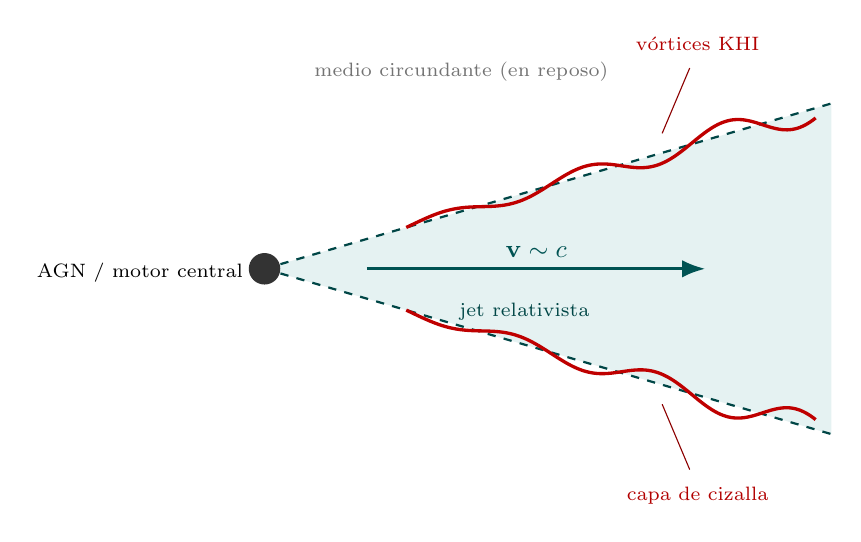
\begin{tikzpicture}[>=Latex,scale=1.0]

% pendiente del borde (cono mas abierto)
\def\m{0.2917}

% --- relleno del jet (cono) ---
\fill[teal!10] (0,0) -- (7.2,2.1) -- (7.2,-2.1) -- cycle;

% --- bordes del jet: rectas punteadas ---
\draw[thick,dashed,teal!55!black] (0,0) -- (7.2,2.1);
\draw[thick,dashed,teal!55!black] (0,0) -- (7.2,-2.1);

% --- oscilacion leve (KHI) a lo largo de cada borde; amplitud crece aguas abajo ---
\draw[very thick,red!75!black,smooth,samples=160,domain=1.8:7.0]
   plot (\x,{ \m*\x + (0.028*\x)*sin(\x*200) });
\draw[very thick,red!75!black,smooth,samples=160,domain=1.8:7.0]
   plot (\x,{-\m*\x - (0.028*\x)*sin(\x*200) });

% --- nucleo / motor central ---
\fill[black!80] (0,0) circle (0.2);
\node[font=\scriptsize,anchor=east] at (-0.15,-0.05) {AGN / motor central};

% --- flujo del jet ---
\draw[->,very thick,teal!65!black] (1.3,0) -- (5.6,0) node[midway,above,font=\small]{$\mathbf{v}\sim c$};
\node[font=\scriptsize,teal!55!black] at (3.3,-0.55) {jet relativista};

% --- etiquetas KHI (fuera de la zona de la onda, con guia) ---
\node[font=\scriptsize,red!70!black,anchor=south] at (5.5,2.65) {v\'ortices KHI};
\draw[red!55!black,thin] (5.4,2.55) -- (5.05,1.72);
\node[font=\scriptsize,red!70!black,anchor=north] at (5.5,-2.65) {capa de cizalla};
\draw[red!55!black,thin] (5.4,-2.55) -- (5.05,-1.72);

% --- medio externo ---
\node[font=\scriptsize,black!55] at (2.5,2.5) {medio circundante (en reposo)};

\end{tikzpicture}
\end{document}
